\begin{frame}{AP Memory Usage Rules}
  \begin{columns}
  \column{0.48\linewidth}
  \begin{outline}
  \1 Input / output must have same lifetime (swap)
  \1 Boundary solves require new input / output 
  \1 Time-cuts can re-use input/ output 
  \1 Periodic solves
  \2 Memory for a complex buffer
  \2 THEN
  \2 Memory for boundary solves
  \2 THEN
  \2 Memory for time-cuts
  \1 Each boundary solve needs a separate memory
  \end{outline}

  \column{0.48\linewidth}
  \begin{center}
  \centering
  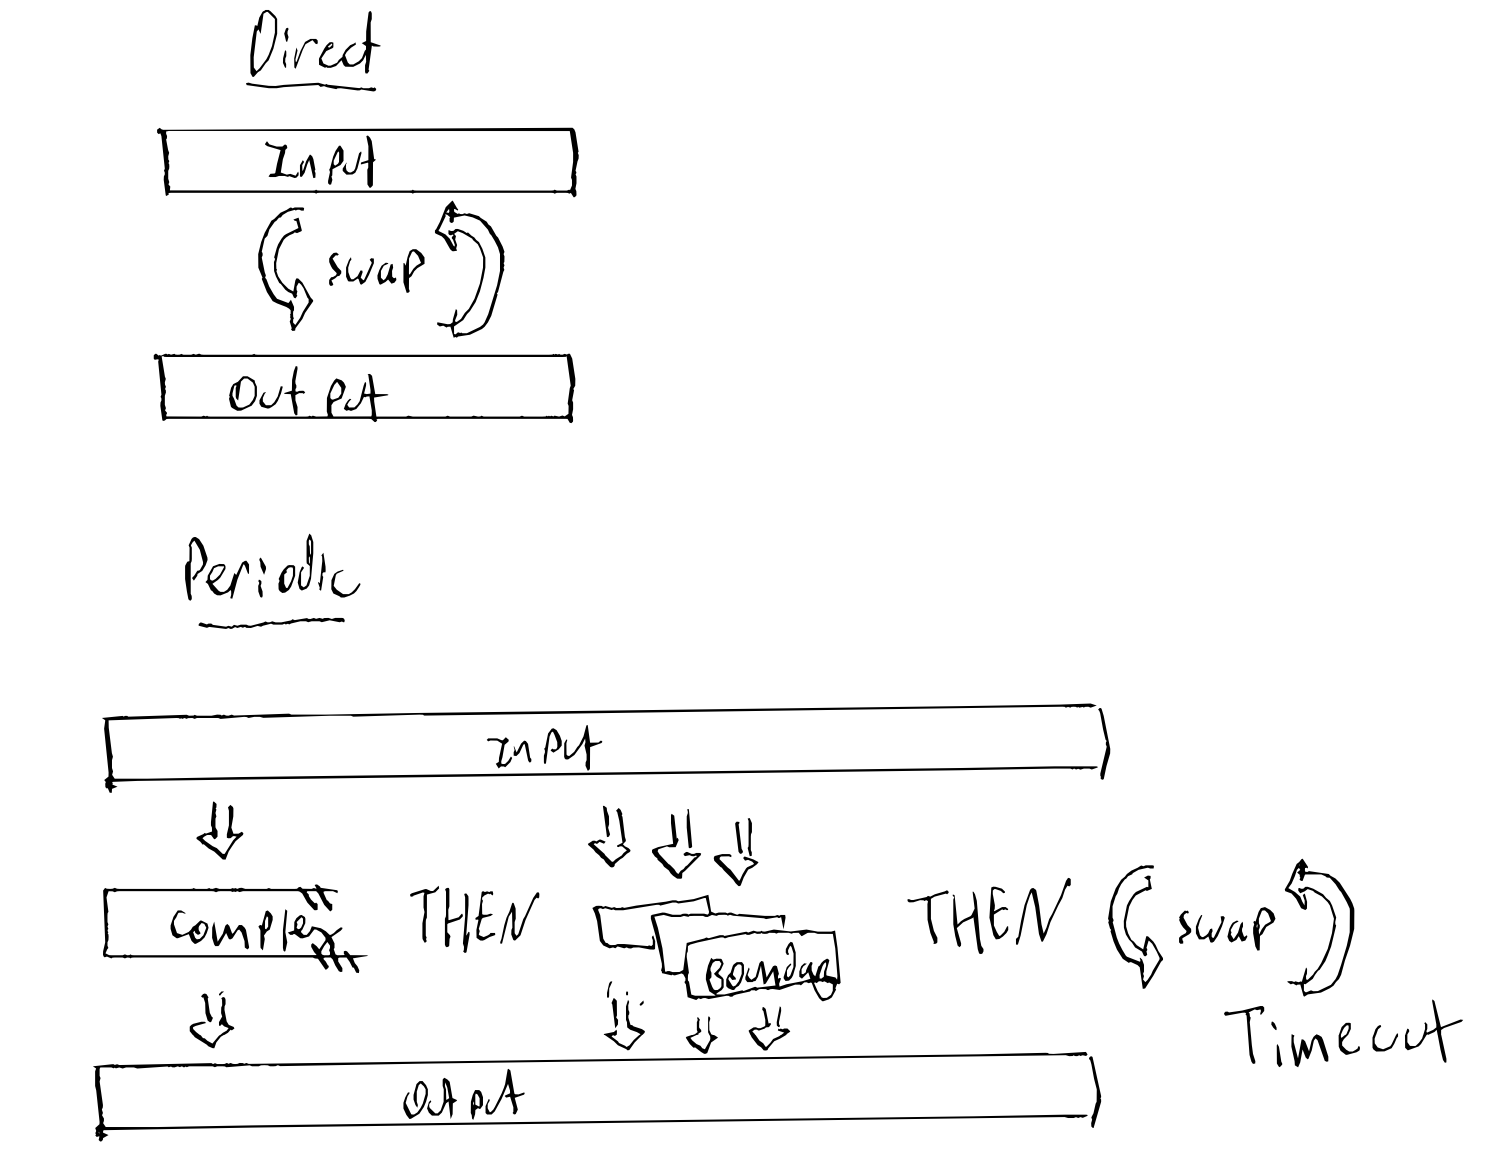
\includegraphics[width=\textwidth]{memory_usage.png}
  \end{center}
\end{columns}
\end{frame}

\begin{frame}{AP Scratch Space}
  \begin{outline}
  \1 Single allocation 
  \1 Pre-compute slices with two passes
  \2 Sum memory requirement for each node
  \2 Calculate memory offset + size for each use
  \1 Requires unsafe Rust
  \1 We guarantee mutually exclusive access
  \1 Must respect alignment for SIMD
  \end{outline}

\begin{center}
  \centering
  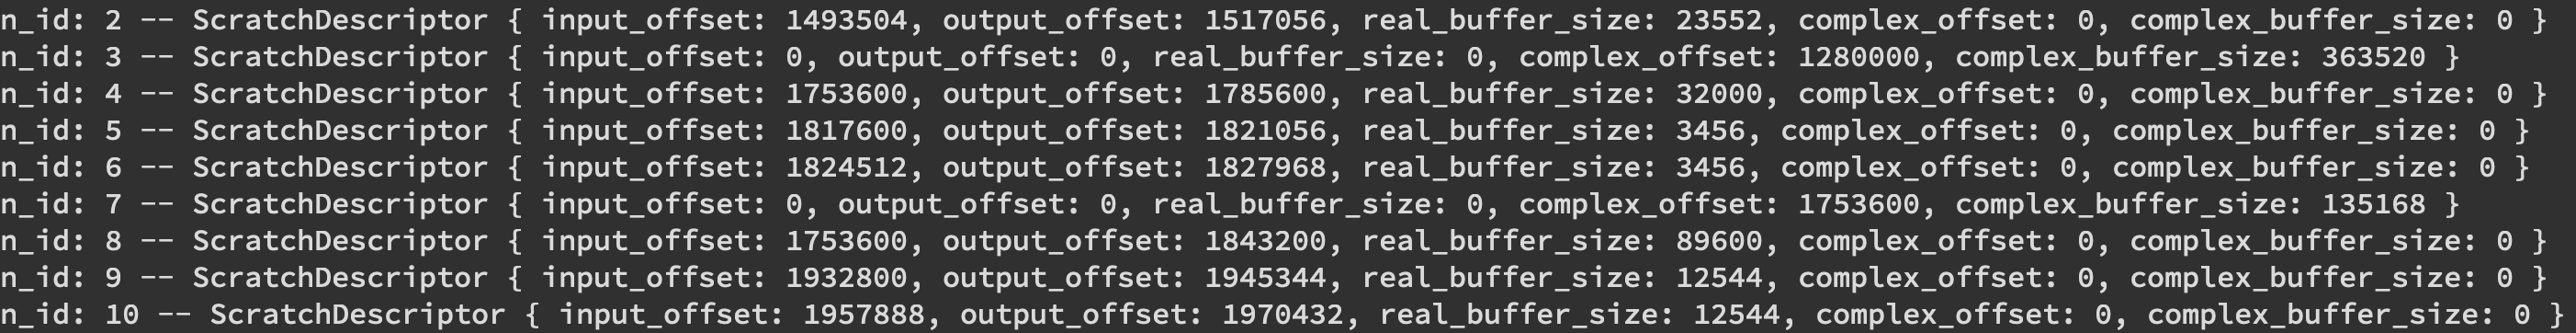
\includegraphics[width=\textwidth]{scratch_d.png}
\end{center}
\end{frame}

\placelogofalse
\begin{frame}{Threading Safety}
  \begin{columns}
  \column{0.48\linewidth}
  \begin{center}
  \centering
  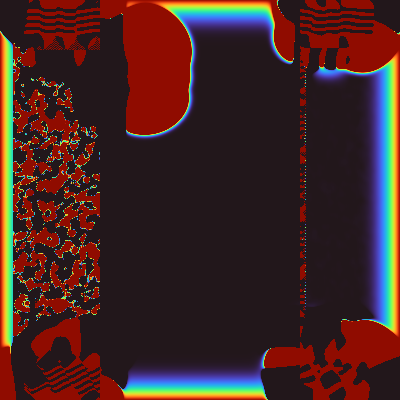
\includegraphics[width=0.6\textwidth]{glitch_01.png}

  \vspace{0.1cm}

  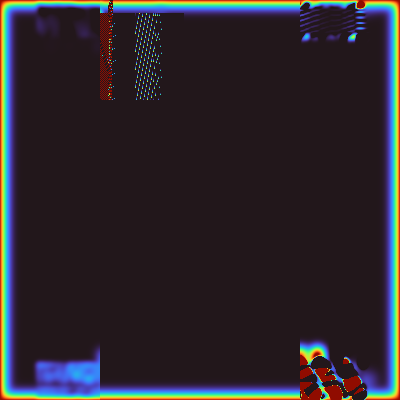
\includegraphics[width=0.6\textwidth]{glitch_02.png}
  \end{center}

  \column{0.48\linewidth}
  \begin{center}
  \centering
  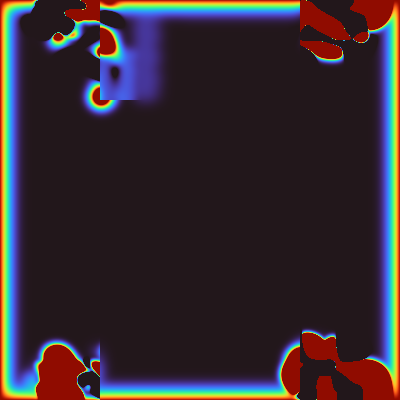
\includegraphics[width=0.6\textwidth]{glitch_03.png}

  \vspace{0.1cm}

  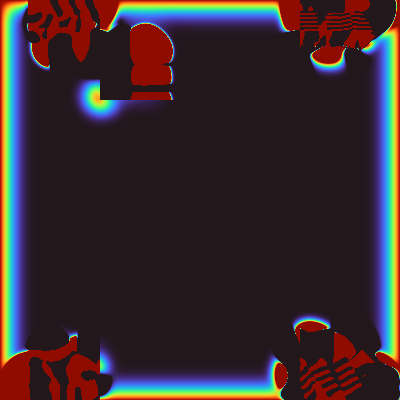
\includegraphics[width=0.6\textwidth]{glitch_04.png}
  \end{center}
\end{columns}
\end{frame}
\placelogotrue
